% Made up for the tikra benchmark.
\usetikzlibrary{decorations.pathmorphing, decorations.pathreplacing}
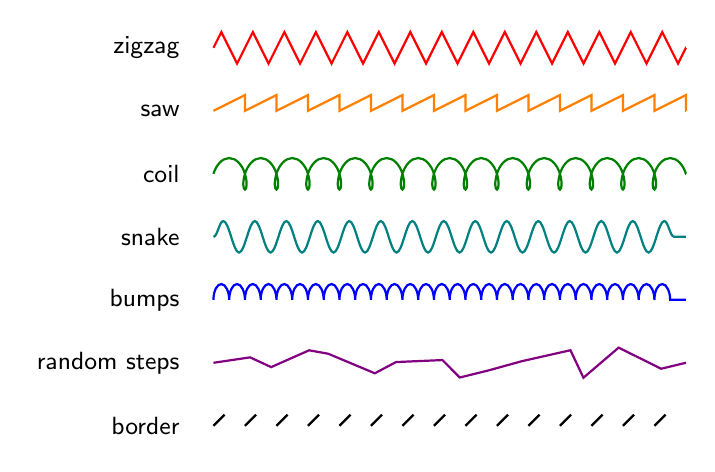
\begin{tikzpicture}[thick, every node/.style={anchor=east, font=\sffamily\small}]
  \foreach \d/\c/\y in {zigzag/red/0, saw/orange/-0.8, coil/green!50!black/-1.6, snake/teal/-2.4, bumps/blue/-3.2, random steps/violet/-4.0, border/black/-4.8} {
    \node at (-0.3,\y) {\d};
    \draw[\c, decorate, decoration={\d, amplitude=2mm, segment length=4mm}] (0,\y) -- (6,\y);
  }
\end{tikzpicture}
